\section*{Brainstorm}
\begin{figure}[H]
	\centering
	\begin{tikzpicture}
	\path[mindmap,
	every node/.style=concept,
	concept color=black,
	scale=0.5,
	text=white,
	text width=2cm,
	grow cyclic,
	level 1/.append style={level distance=8.5cm,sibling angle=70},
	level 2/.append style={level distance=6cm,sibling angle=45}]
	node[concept] {Simple sketch to virtual world}
	[clockwise from=-20]
	child[concept color=green!50!black] {
		node[concept] {Building}
		[clockwise from=-20]
		child { node[concept] {Over construction} }
		child { node[concept] {Overuse of materials} }
	}  
	child[concept color=black!20!blue] {
		node[concept] {Architecture}
		[clockwise from=-67]
		child { node[concept] {Sketching} }
		child { node[concept] {3D modeling} }
	}
	child[concept color=orange] { node[concept] {Presentation} [clockwise from=-90]
		child { node[concept] {Teachers}}
		child { node[concept] {Students}}
	};
	\end{tikzpicture}
	\captionof{figure}{The outcome of the intitial brainstorm}
	\label{fig:brainstorm}
\end{figure}
\section*{Interview Questions for plant center customers}\label{sec:interviewQuestionsCustomer}
% when and where
% what does location and time mean for the data
List of questions for target group
\begin{itemize}
	\item[-] Have you ever used a garden designer?
	\item[-] What was your experience?
	\item[-] What are you planning to buy?
	\item[-] What are you plan/thoughts for when you buy a new plant?
	\item[-] What do you consider when you buy a new item for your garden?
	\item[-] How often do you make major changes to your garden?
	\item[-] For which reasons did you decide to purchase this item?
	\item[-] What was the latest item you bought that you were not satisfied with?
	\item[-] Do you have a garden?
	\item[-] How did you start the design process?
	\item[-] What tools did you use, if any?
	\item[-] When did you make changes to your garden?
	\item[-] What big changes would you like to make?
	\item[-] Are you retired?
	\item[-] If you had all the time in the world, what would you change about your garden?
	\item[-] Do you enter the garden center with a budget in mind?
	\item[-] Why are you here? \\
\end{itemize}

\paragraph*{Demographic information}
\begin{itemize}
	\item[-] Sex
	\item[-] Age
	\item[-] Job
	\item[-] Marital Status
	\item[-] Level of education
\end{itemize}


\section*{Interview Questions for experts}\label{sec:interviewQuestionsExperts}
This is a rough outline of the questions we asked the experts. The translated version (and the original Danish version) of each question is listed below. Since the interview was semi-structured all questions were not necessarily used or not used in exactly in the form written here.\\

Personal questions:
\begin{itemize}
	\item[-] How did you end up in this business? (Hvordan er du endt i den her branche?)
	\item[-] What is your role in the company? (Hvad er din rolle i virksomheden?)
	\item[-] What does your workday consist of? (Hvad består din arbejdsdag af?)\\
\end{itemize}

Design questions:
\begin{itemize}
	\item[-] How large of a garden area do you usually work with? (Hvor stort haveareal arbejder I med normalt?)
	\item[-] What plants, trees or other elements are trending at the moment? (Hvilke planter, træer eller andre have elementer, hitter lige nu?)
	\item[-] What is a popular garden style? (Hvad er en populær have stil?)
	\item[-] Do many people want to have a lake or a fishpond built in the garden? (Er der mange der får lavet søer eller fiskedamme i haven?)
	\item[-] What do you need to be specifically aware of when designing garden in Denmark? (Hvad skal man være specielt opmærksom på når man designer haver i Danmark?)
	\item[-] How do you show/demonstrate a final design for the clients? (Hvordan viser/demonstrere du færdige designs til kunderne?)\\
\end{itemize}

Target group questions:
\begin{itemize}
	\item[-] What kind of people do usually contact you? (Hvilke mennesker henvender sig mest til jer/dig?)
	\item[-] What is the most usual demography? (Hvad er den mest almindelige demografi?)
	\item[-] Is it usually private clients or is it municipal clients (Er det primært privatpersoner eller er det kommuner, der er jeres kunder?)
	\item[-] Do people need designing for the whole garden or just parts of their garden? (Skal folk have lavet hele haven eller er det kun dele af haven?)
	\item[-] Who makes the 3D visualization of the garden? Is it something you create internally in the company, or does it come from outside cooperators? 
	\item[-] How much influence do the clients have in the process? (Hvor meget indflydelse har kunderne i processen?)\\
\end{itemize}

Technology questions:
\begin{itemize}
	\item[-] Do you offer 3D visualization of the gardens? (Tilbyder du/i 3D visualisering af haverne?)
	\item[-] Who is doing the 3D visualization of the garden? Are you doing it internally in the company or does it come from outside? (Hvem laver 3D visualiseringen af haven? Er det noget i laver internt i virksomheden, eller kommer det udefra?)
	\item[-] Why did you choose to offer this? (Hvorfor valgte i at tilbyde dette?)
	\item[-] For how long have you been offering this? (Hvor lang tid har i tilbudt dette?)
	\item[-] Do people take the offer on 3D visualization of their garden? (Benytter folk sig af tilbuddet om 3D visualisering af haven?)
	\item[-] Can you see the development over time? (Kan man se udviklingen over tid?)
	\item[-] Does this mean that the growth can be followed year by year, or is it about the seasons? (Betyder det at væksten kan følges år for år, eller handler det om årstider?)
	\item[-] Is it something people make use of?\\
\end{itemize}

Project specific questions:
\begin{itemize}
	\item[-] How do you think a Virtual Reality experience in the 3D environment would be received? (Hvordan tror du at en VR oplevelse i 3D miljøet, ville blive modtaget?)
	\item[-] Is this a product that would be interesting for you in your process and how do you see this working? (Er det et produkt, der ville være interessant for jer, i jeres process, og hvordan forestiller du dig at det ville fungere?)\\
\end{itemize}

SOTA questions:
\begin{itemize}
	\item[-] Have you heard of this type of product before or something similar? (Har du hørt om denne type produkt før eller noget lignende?)
\end{itemize}

\section*{Interview transcriptions}\label{interviewTranscriptions}
Due to the large number of pages these transcriptions have not been included in this report. We refer you to the digital appendices.
\begin{comment}
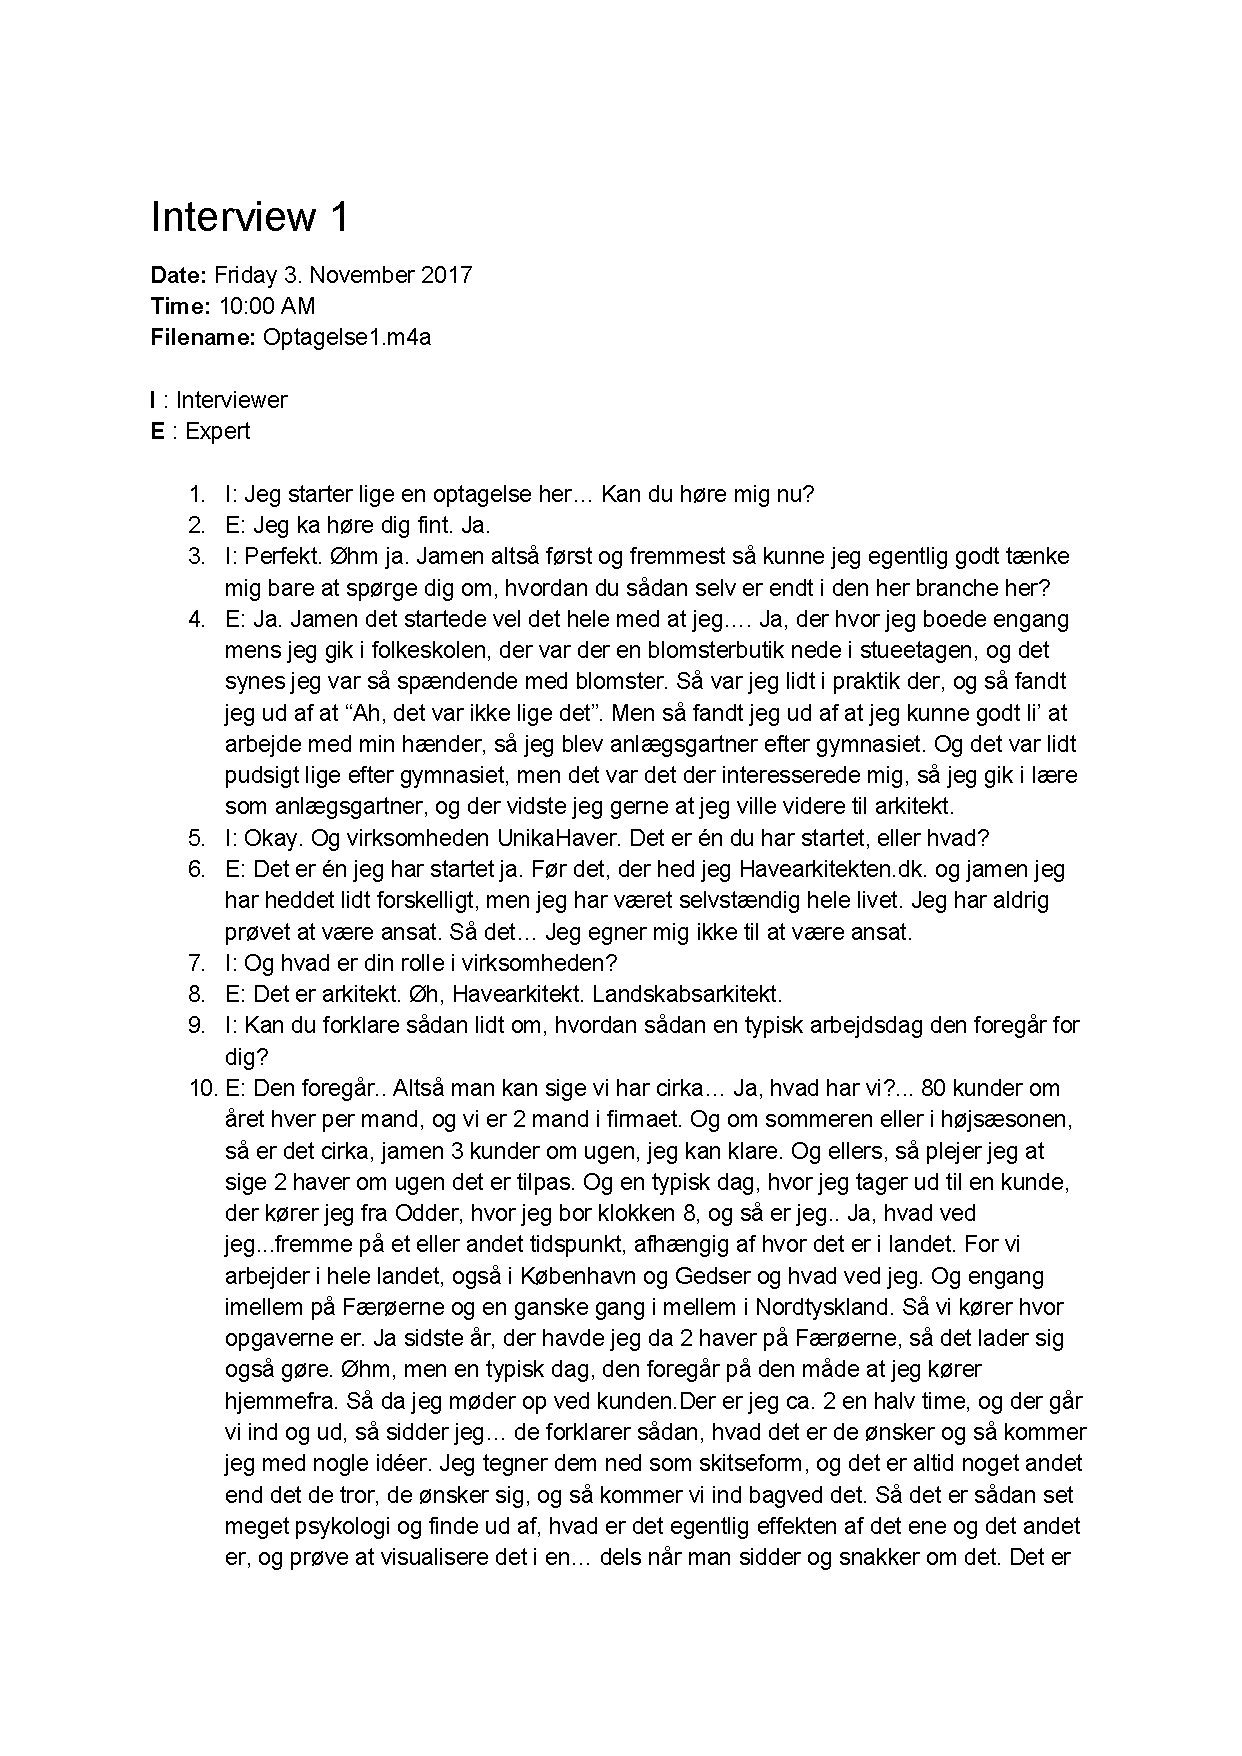
\includepdf[pages=-]{figure/Appendices/transcribedInterview1.pdf}
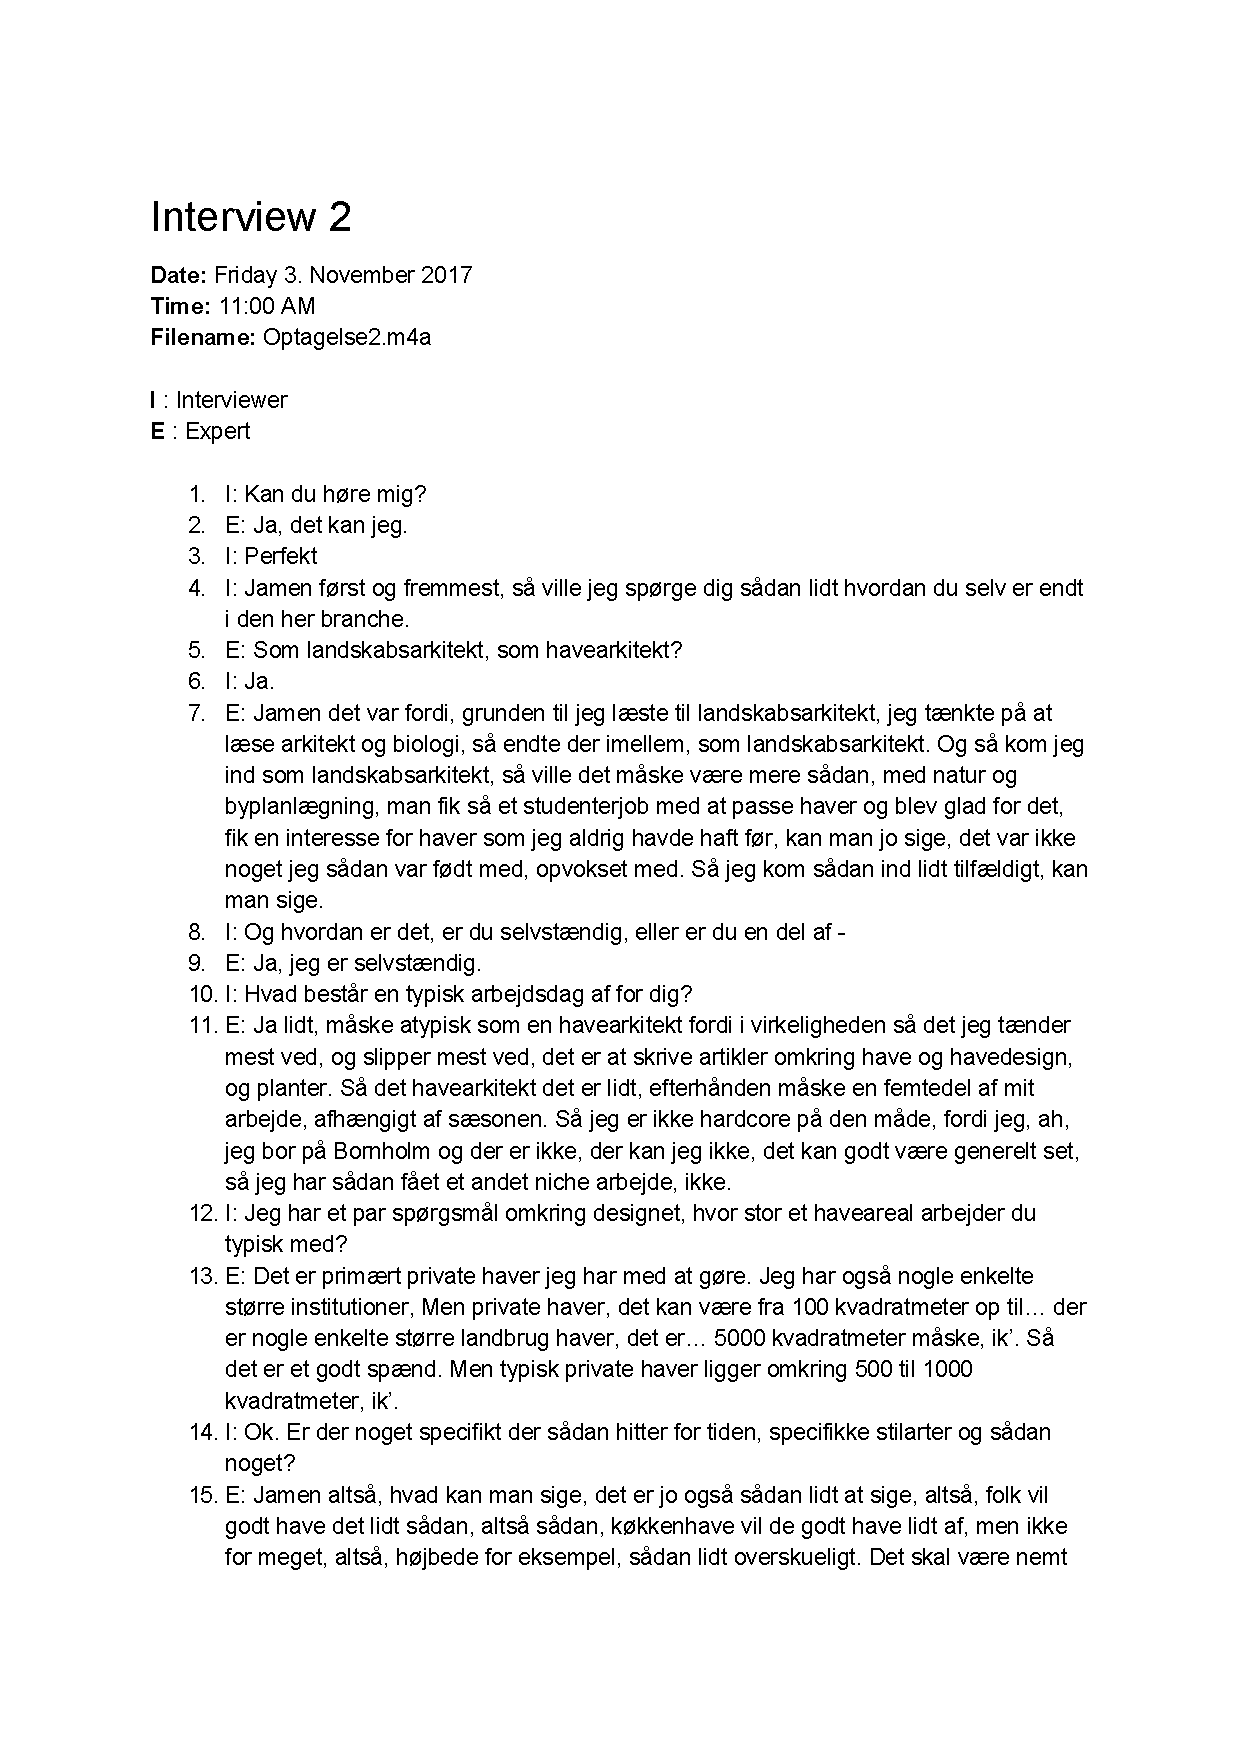
\includepdf[pages=-]{figure/Appendices/transcribedInterview2.pdf}
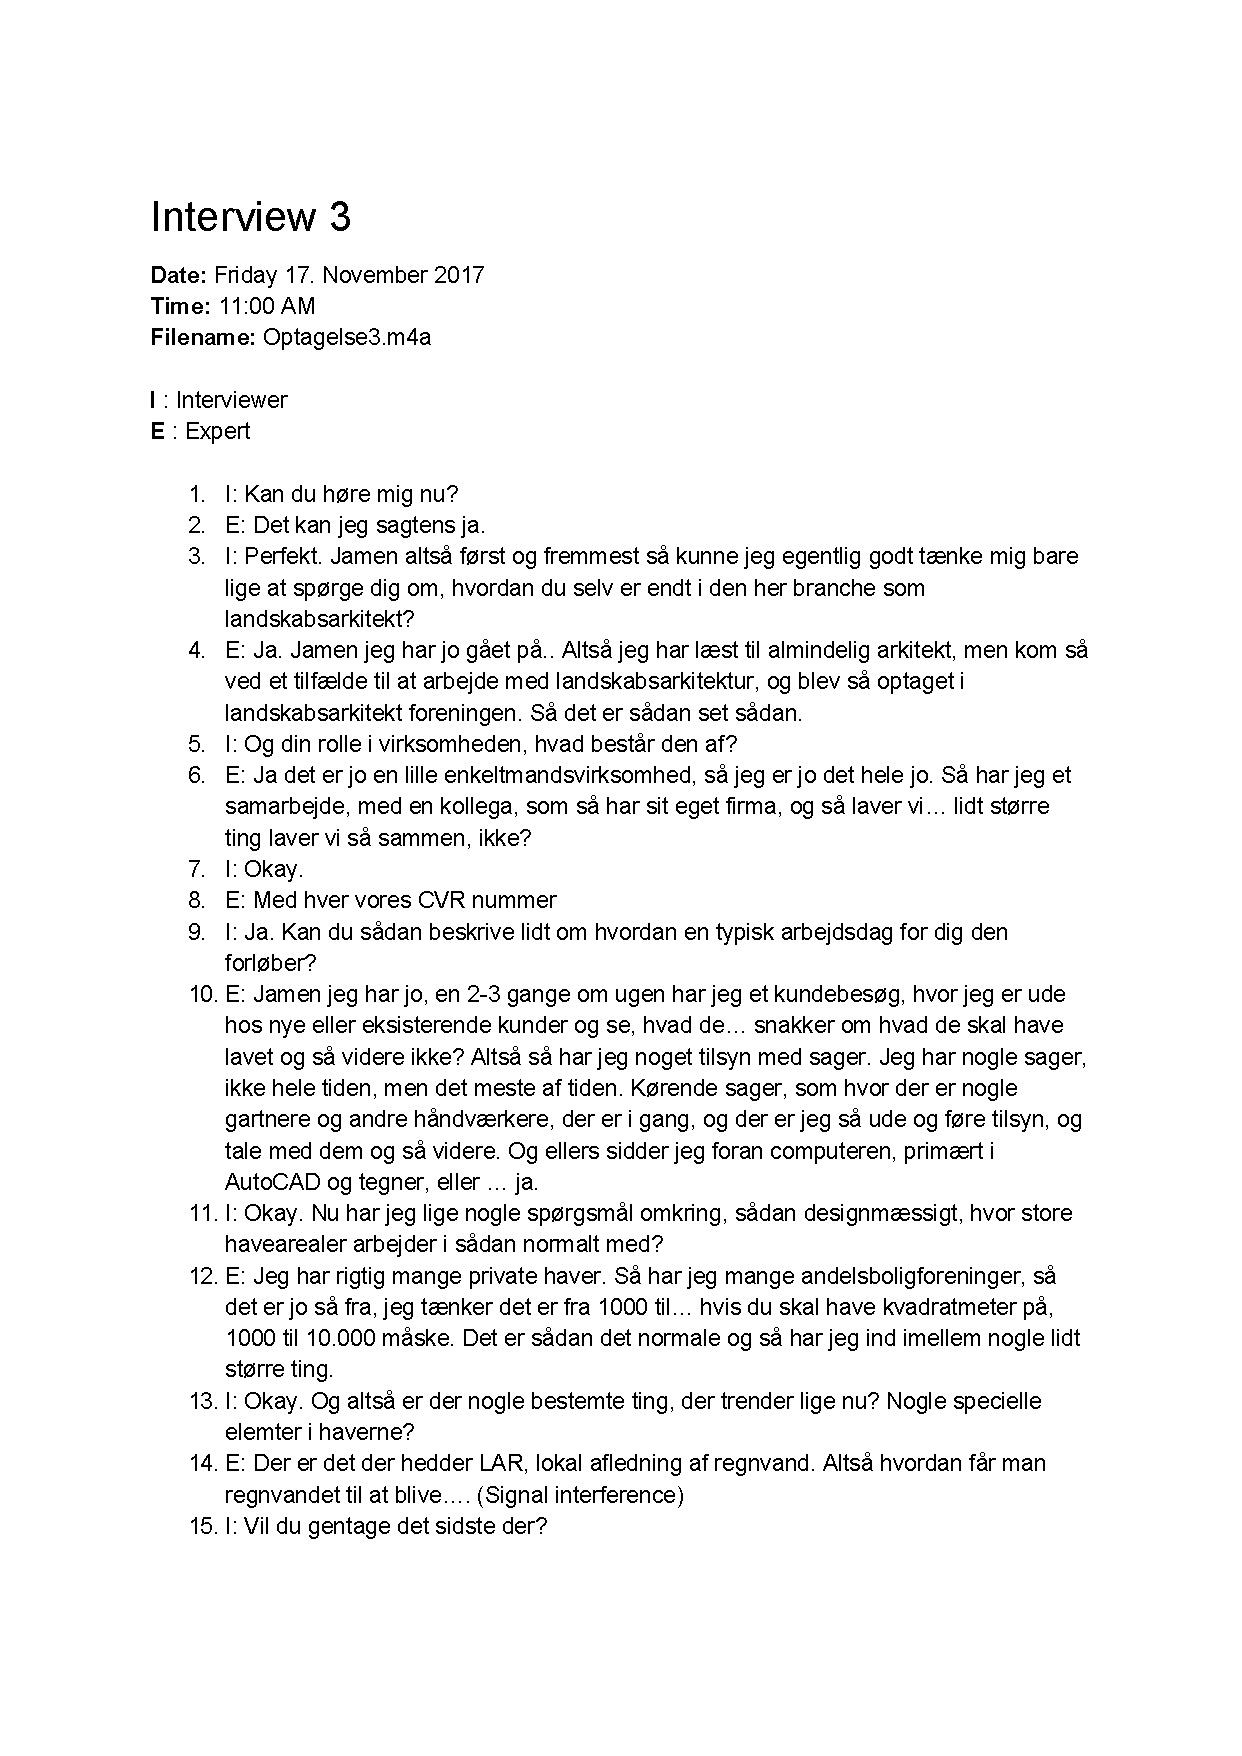
\includepdf[pages=-]{figure/Appendices/transcribedInterview3.pdf}
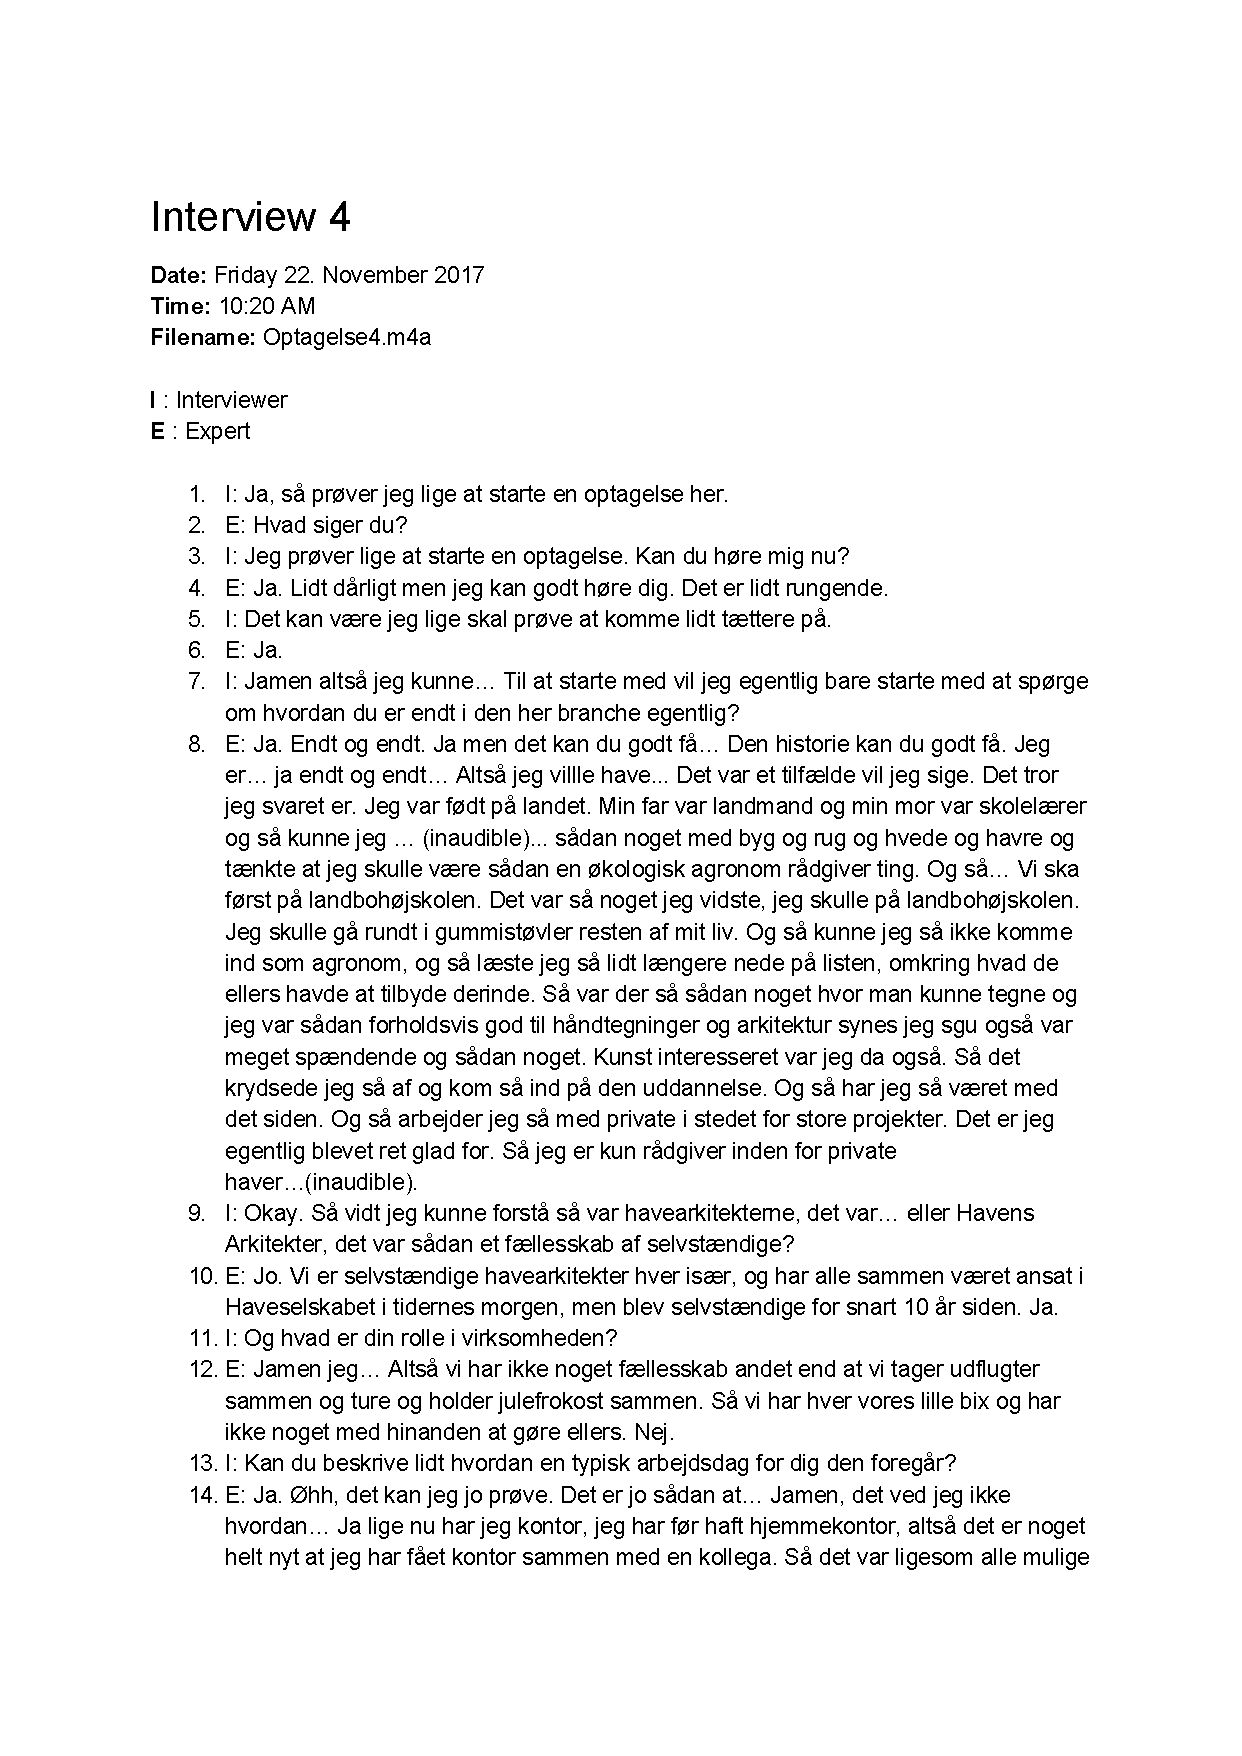
\includepdf[pages=-]{figure/Appendices/transcribedInterview4.pdf}
\end{comment}
\section*{Marker auto-generating program}
The code shown in Listing \ref{listing:generatorCode} is the Processing code used to generate markers given just an integer array as input. The program was developed using Processing.

\begin{listing}[H]
	\caption{Code for the marker auto-generating program}
	\label{listing:generatorCode}
	\begin{minted}[frame=lines,
		framesep=2mm,baselinestretch=1.1,fontsize=\footnotesize,linenos]{java}
int[] markers = {1, 2, 4, 8,16,32,64,128,100,3,9};
int spacing = 800;
PImage circle;
PImage values[] = new PImage[8];
void setup() {
	circle = loadImage("circle.png");
	for (int i = 0; i<values.length; i++) {
		values[i] = loadImage(""+int(pow(2, i))+".png");
	}
	size(3508, 4961);
	surface.setVisible(false);
	background(255);
	//4x6 markers on a3 paper
	int x = 0;
	int y = 0;
	int counter=0;
	for (int i = 0; i<markers.length; i++) {
		drawMarker(markers[i], x, y);
		x++;
		if (x>3) {
			x = 0;
			y++;
			if(y>4){
				save("result"+counter+".png");
				counter++;
				x=0;
				y=0;
				
			}
		}
	}
	save("result"+counter+".png");
	exit();
}

void drawMarker(int num, int xpos, int ypos) {
	int x = spacing/2+xpos*spacing;
	int y = spacing/2+ypos*spacing;
	String str = binary(num, 8).toString();
	int s = int(circle.width*1.5);
	image(circle, x, y,s,s);
	
	for (int i = 0; i<8; i++) {
		if (str.charAt(i)=='1') {
			tint(0,255);
			image(values[7-i], x, y,s,s);
			tint(255);
		}
	}
	
}
	\end{minted}
\end{listing}

